%%%%%%%%%%%%%%%%%%%%%%%%%%%%%%%%%%%%%%%%%
% Reporte de prácticas
% Ingeniería Informática
% LaTeX Template
% Version 0.1 (27/09/20)
% Original author: Abraham Marianjel Sepúlveda
%%%%%%%%%%%%%%%%%%%%%%%%%%%%%%%%%%%%%%%%%%
\documentclass[12pt,letterpaper]{article} 
\usepackage[utf8]{inputenc} 
\usepackage[spanish, es-tabla, es-nodecimaldot]{babel} % Formato a español
\usepackage[T1]{fontenc}    % Permite utilizar otras tipografías
\usepackage[vmargin=2.5cm,hmargin=2.5cm]{geometry}
\usepackage{multicol}   % Unir columnas en tablas y formato a dos columnas
\usepackage{multirow}   % Unir filas en tablas
\usepackage{graphicx}   % Necesario para insertar gráficas
\usepackage{float}      % Corregir ubicación de imágenes y tablas
%\usepackage{subfigure} % Insertar subfiguras
\usepackage{url}       % Hiervínculo a direcciones URL
\usepackage{cite}
\usepackage{lscape} % Para poner una unica hoja en horizontal
\usepackage{listings}
\usepackage{flushend}
\usepackage[none]{hyphenat} % Permite utilizar el comando \sloppy
\usepackage[small]{caption}	% Reduce el tamaño de letra utilizado en los pies de figura.
\usepackage{hyperref}   % Agrega enlaces internos de las secciones, figuras y tablas.
\usepackage{color}      % Definición de colores
    \hypersetup{colorlinks=true, linkcolor=[rgb]{0,0,1}, citecolor=[rgb]{0,0,1}}
\usepackage{xcolor}		% Permite definir un color para utilizarlo dentro del documento.
    \definecolor{gris}{RGB}{70,70,70}	% Definiendo el color gris
    \definecolor{negro}{RGB}{40,40,40}		% Definiendo el color negro

%%%%%%%% Modificación de los espacios de los títulos de secciones %%%%%%%%%%
%======================================================================================
\usepackage{titlesec}		% Permite reconfigurar  los títulos de las secciones y subsecciones
%\renewcommand\thesection{\Roman{section}}	% Numeración romana en las secciones
\renewcommand\thesubsection{\Roman{subsection}}		% Numeración romana en las subsecciones
\titlespacing*{\section}{0pt}{2.5mm}{0mm}	% Espaciado del título {espacio izquierdo}{arriba del título}{abajo del título}
\titleformat{\section}[block]{\large\scshape\centering}{\thesection.}{1em}{}	% Espaciado del título de las secciones
\titleformat{\subsection}[block]{\large}{\thesubsection.}{1em}{}				% Espaciado del título de las subsecciones
%%%%%%%%%%%%%%%%%%%%%%%%%%%%%%%%%%%%%%%%%%%%%%%%%%%%%%%%%%%%%%%%%%%%%%%%%%%%%%

%Se define un comando \colorhrule para hacer líneas horizontales de color con 3 argumentos: color, largo, ancho.
\newcommand{\colorhrule}[3]{\begingroup\color{#1}\rule{#2}{#3}\endgroup}

\setlength{\intextsep}{1mm} % Distancia superior e inferior en objetos flotantes
\setlength{\columnsep}{5mm} % Separación entre columnas del documento
%**************************************Encabezado****************************************
%=========================================================================================
\begin{document}
\sloppy     % Evita que las palabras se corten al saltar de línea.
\begin{center}
	\begin{tabular}{cc}
	\multirow{2}{3.5cm} {
\includegraphics[scale=0.3]{../../../Logos FACE/logosimbologia.png}   }	& \huge{\textsc{\textbf{Universidad del Bio Bio}}}\\ %\vspace{5mm}
 & \scriptsize{\textsc{Facultad de Ciencias Empresiariales}}\\[4mm]% Sele puede cambiar al LARGE
 & \Large{\textsf{\textbf{Guía BPMN y Diagrama de Clases}}}\\
 & \small Profesor: {\textsf{Luis Rojas}}\\
 & \small Ayudante: {\textsf{Abraham Marianjel}}\\

 & \small{\textsc{Ingeniería Civil en Informática $|$ Modelamiento}}\\
 & \today\\
	\end{tabular}
\end{center}
\begin{center}
\colorhrule{negro}{16.5cm}{1.2pt}
\end{center}


\noindent 
\section{Actividad de Ejemplo}
\subsection{Enunciado}
Se desea modelar el funcionamiento de un aparcamiento público de automóviles. Cuando unconductor se acerca a la máquina situada en la entrada, debe pulsar un botón para obtener el resguardo de aparcamiento, una cámara graba la matrícula que se almacena en el resguardo junto a la hora de entrada. Cuando el resguardo es retirado se abre la barrera de entrada la cual se cierra unos instantes después de detectar el paso del vehículo. Para salir del aparcamiento los conductores primero abonan el importe asociado a la estancia en un cajero automático, éste graba la hora de pago en el resguardo de aparcamiento, dejando un margen de 10 minutos para abandonar las instalaciones. Para salir de una manera efectiva el conductor introduce en la máquina situada en la salida el resguardo de aparcamiento, en ese momento el sistema lee la matrícula del vehículo, comprueba la hora de pago y levanta la barrera de salida, la cual se cierra unos instantes después de detectar el paso del vehículo. El aparcamiento funciona también para abonados, los cuales para entrar y salir del aparcamiento deben introducir una tarjeta magnética. En la tarjeta se graba la matrícula al entrar y se comprueba a la salida. Para facilitar el pago de los conductores no abonados se desea implantar un sistema por telefonía móvil que mediante mensajes SMS permita pagar la estancia en el aparcamiento. Al entrar el usuario recoge el ticket de entrada y para salir envía un mensaje SMS con el número de ticket, el importe se carga en la factura de teléfono. El sistema informático del aparcamiento recibe el mensaje SMS de confirmación del pago. Para salir el conductor introduce el ticket de entrada y pulsa un botón de la máquina que indica pago telefónico, el sistema comprueba si el usuario ha enviado el mensaje SMS, en cuyo caso abre la barrera de salida. En este caso se aplican también los 10 minutos de margen para abandonar las instalaciones.\\

\subsection{BPMN}
	\begin{figure}[H]
		\centering
		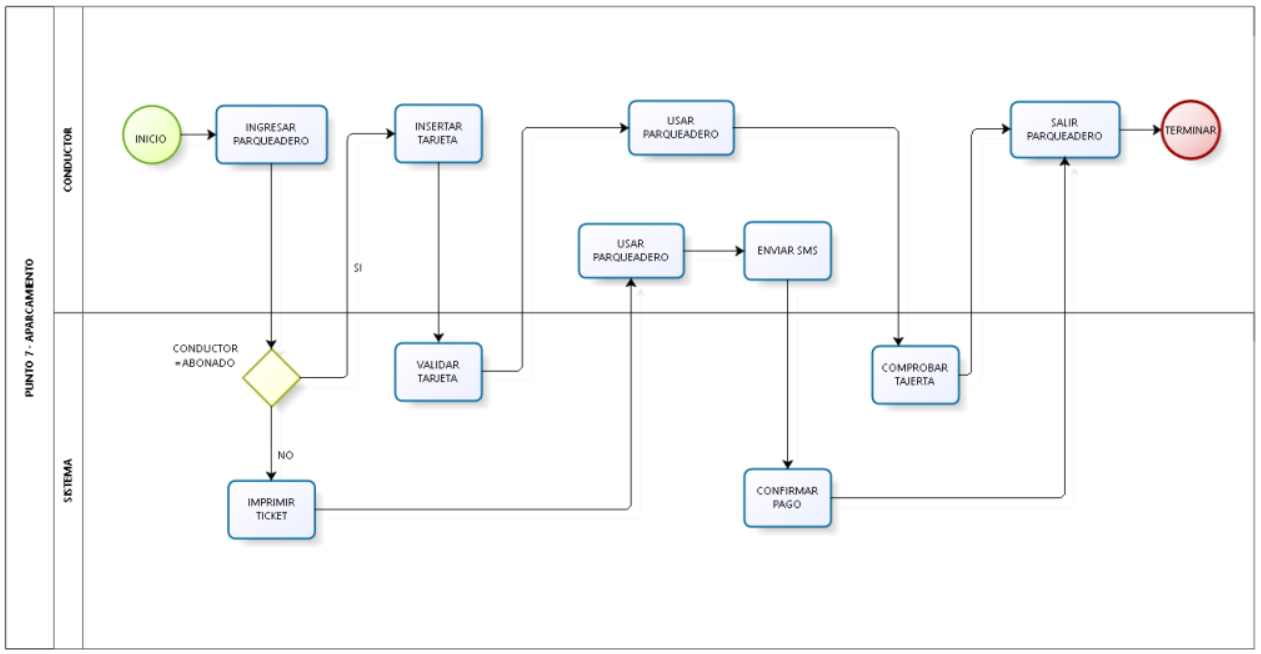
\includegraphics[scale=0.5]{img/ejemplobpmn.PNG}    
		\caption{BPMN }
	\label{fig:rc}
	\end{figure}
	\vspace{1cm}

\subsection{Diagrama de Clases}
	\begin{figure}[H]
		\centering
		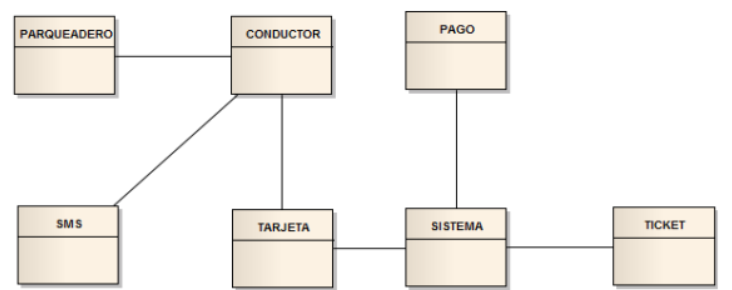
\includegraphics[scale=0.8]{img/ejemploclase.PNG}     
		\caption{Clase }
	\label{fig:rc}
	\end{figure}
	\vspace{1cm}


\subsection{Glosario}
	\begin{figure}[H]
		\centering
		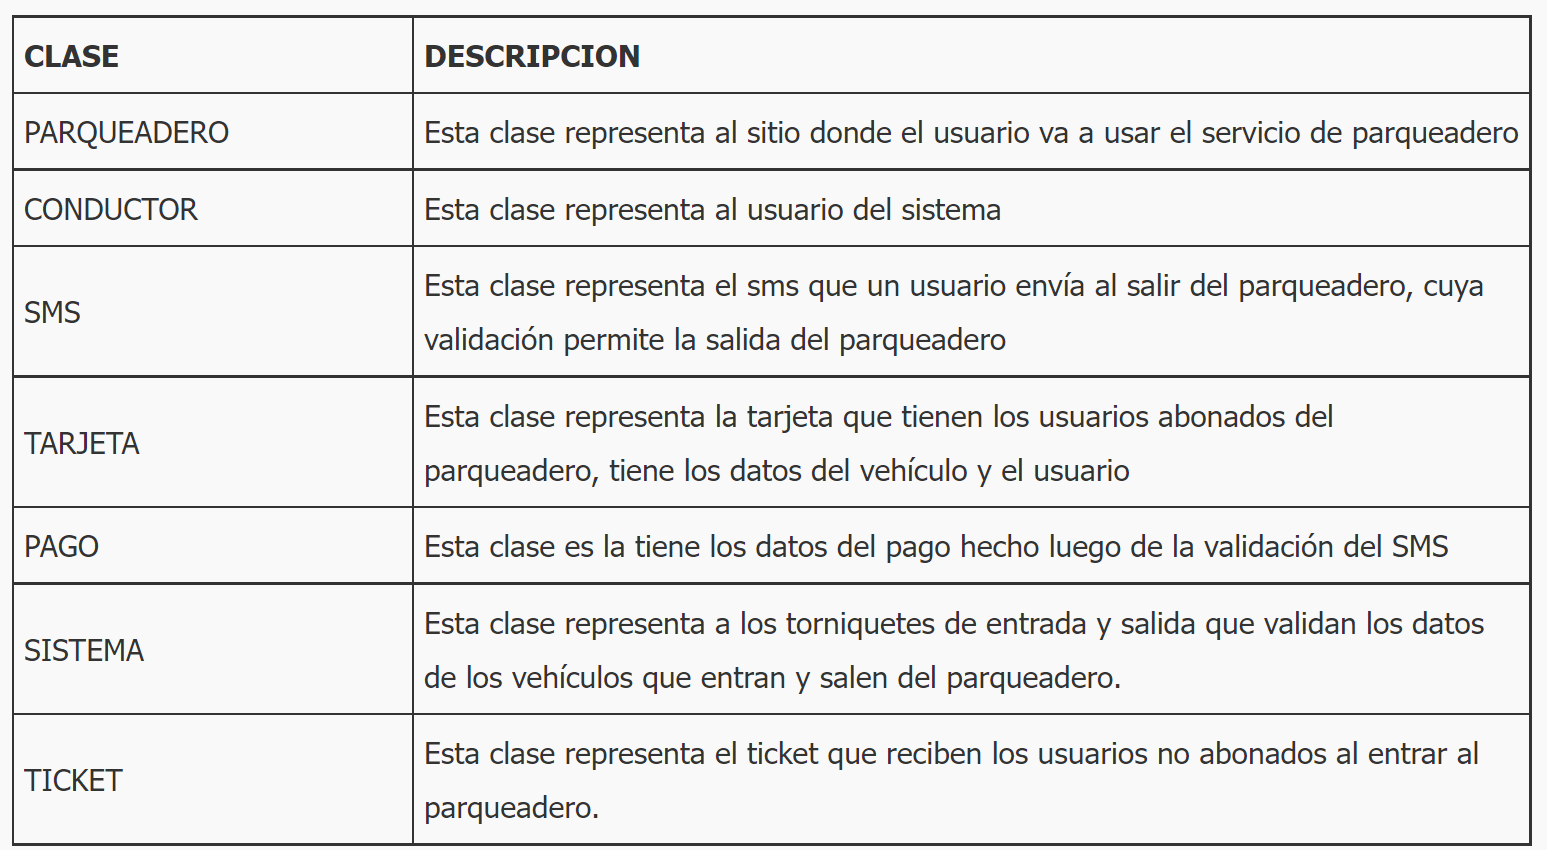
\includegraphics[scale=0.4]{img/ejemploglosario.PNG}    
		\caption{Glosario }
	\label{fig:rc}
	\end{figure}
	\vspace{1cm}


\begin{center}
\vspace{-5mm}
\colorhrule{gris}{16.5cm}{0.7pt}
\end{center}
%*******************************Texto del Informe*********************************************
%==============================================================================================

\section{Actividades}

\subsection{\textbf{Ejercicio 1}}
Complete el siguiente proceso de colaboración entre un cliente y una empresa de venta por catálogo. El cliente lleva a cabo las siguientes actividades (no necesariamente en este orden): pide un artículo, paga el artículo y pregunta sobre el estado de su pedido (el cliente pregunta una vez realizado el pedido cada 3 días si no ha recibido el encargo). En la compañía de ventas existen 3 roles: encargado de pedidos, almacén y contabilidad. El primero recibe los pedidos de artículos, y tranquiliza al cliente cuando éste pregunta por el estado de su encargo, en almacén se prepara la entrega y se envía al repartidor (una empresa externa) y el repartidor la entrega y recibe el pago. El último rol de la compañía es contabilidad que registra los envíos y los pagos. Complete el diagrama inferior, indicando la estructura de control, los mensajes necesarios y las puertas.\\

	\begin{figure}[H]
		\centering
		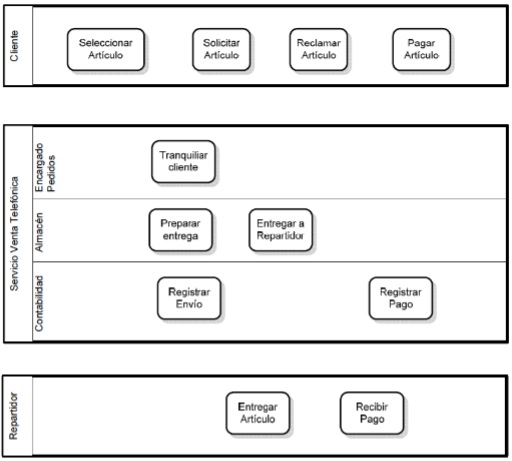
\includegraphics[scale=0.7]{img/ej1.jpg}     
		\caption{Tienda en linea - BPMN }
	\label{fig:rc}
	\end{figure}
	\vspace{1cm}
	
\subsection{\textbf{Ejercicio 2}}
	\begin{figure}[H]
		\centering
		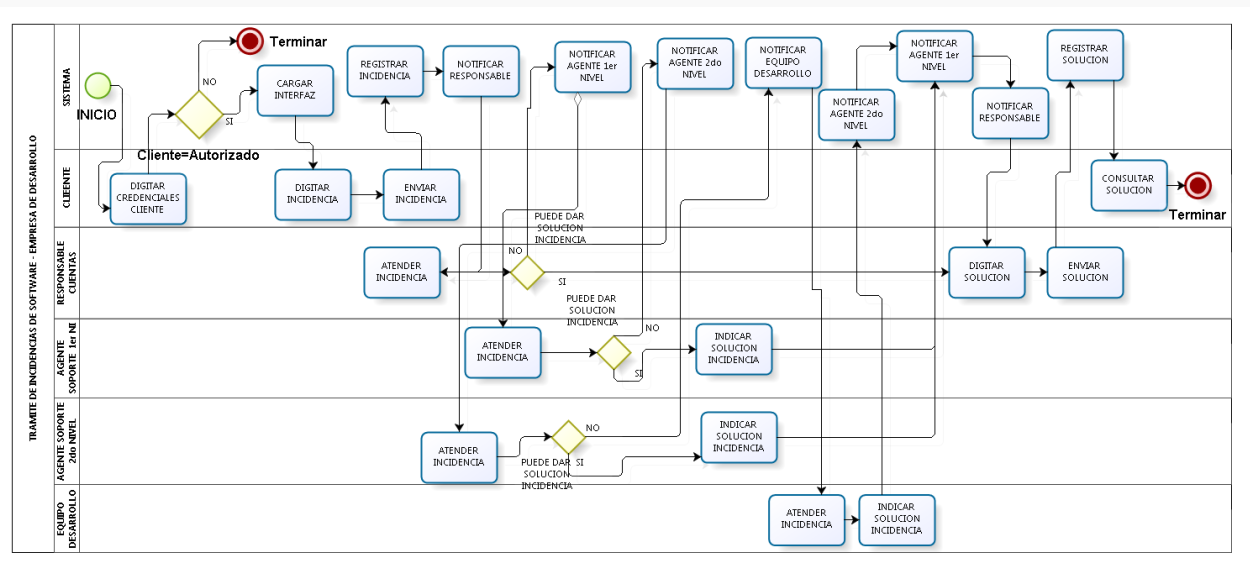
\includegraphics[scale=0.5]{img/ej2.PNG}     
		\caption{Responsables}
	\label{fig:rc}
	\end{figure}
	\vspace{1cm}
	\begin{figure}[H]
		\centering
		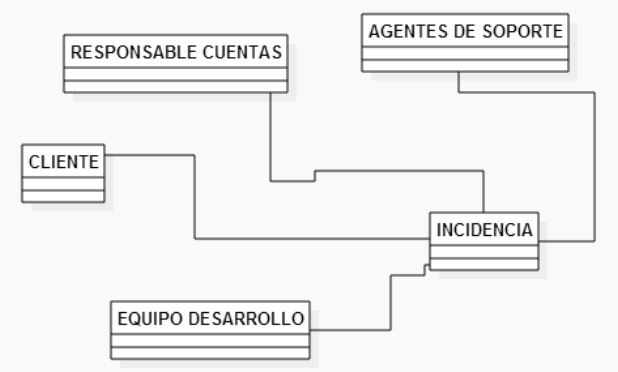
\includegraphics[scale=1]{img/ej22.PNG}     
		\caption{Responsables - Diagrama de Clases}
	\label{fig:rc}
	\end{figure}
	\vspace{1cm}


\subsection{\textbf{Ejercicio 3}}
Se pretende modelar el proceso de gestión de reclamaciones en una compañía aseguradora. Cuando se recibe una reclamación, ésta se registra en el sistema. Después del registro, la reclamación se clasifica en uno de los dos siguientes tipos: simple o compleja. Si la reclamación queda clasificada como simple se comprueba el seguro del cliente, para reclamaciones complejas se comprueba independientemente el seguro y el daño en el vehículo. Después de la comprobación o comprobaciones se genera una resolución de la reclamación, que puede ser positiva o negativa. Si la resolución es positiva se informa al garaje para autorizar la reparación y se planifica el pago al mismo. Para cualquier tipo de resolución (positiva o negativa) se envía una carta al cliente y el proceso termina.\\

	\begin{figure}[H]
		\centering
		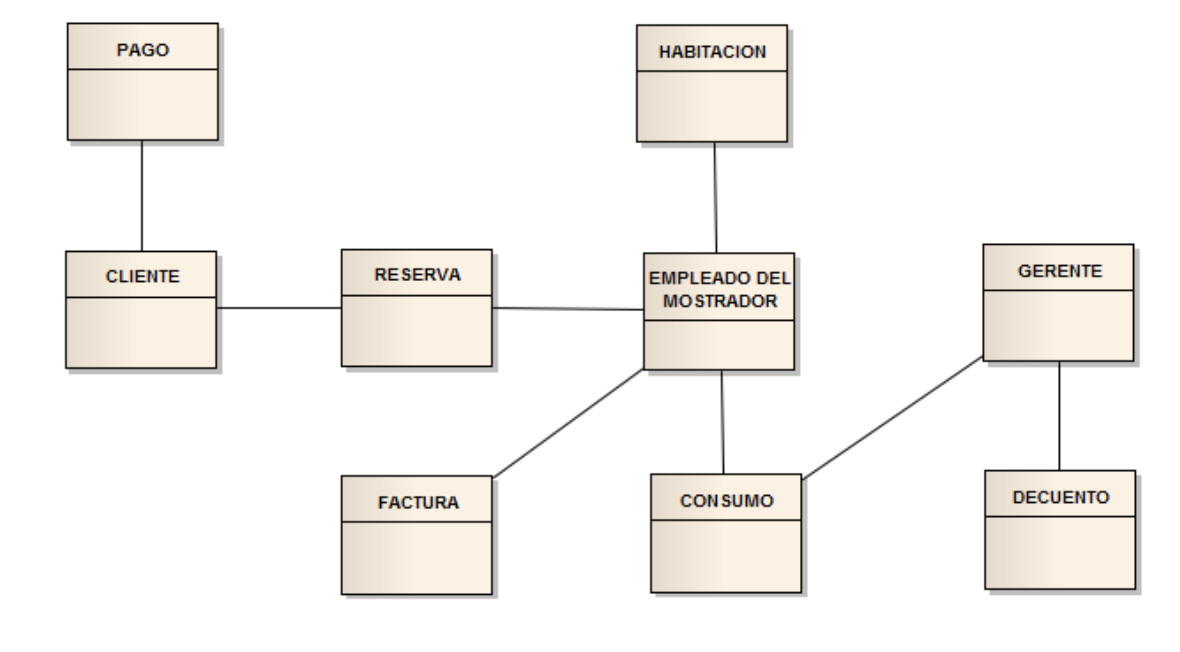
\includegraphics[scale=0.2]{img/ej3.PNG}    
		\caption{Gestion de Reclamos - Diagrama de Clases }
	\label{fig:rc}
	\end{figure}
	\vspace{1cm}
	
\subsection{\textbf{Ejercicio 4}}
 	\begin{figure}[H]
		\centering
		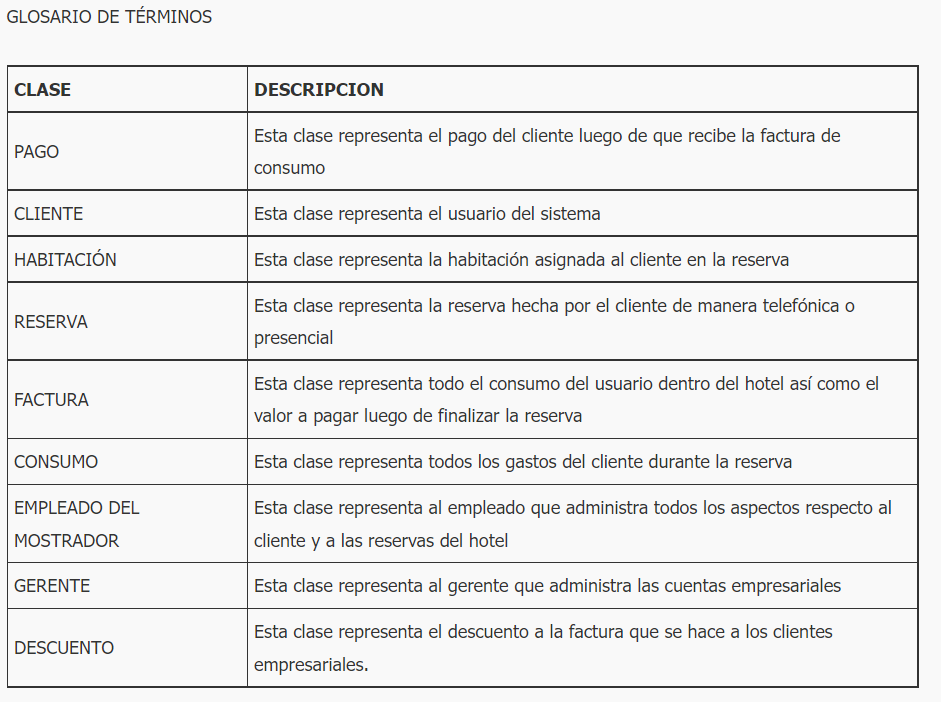
\includegraphics[scale=0.4]{img/ej4.PNG}    
		\caption{Gestion de Reclamos - Diagrama de Clases }
	\label{fig:rc}
	\end{figure}
	\vspace{1cm}

\subsection{\textbf{Ejercicio 5}}
La compañía de metro de la ciudad de Valencia desea implantar una tarjeta inteligente (smart‐card) que facilite la adquisición de billetes y el desplazamiento de los viajeros por las distintas líneas de metro de la ciudad. La tarjeta puede adquirirse en máquinas expendedoras situadas en las distintas estaciones. Los viajeros indican el saldo con el cual quieren cargar la tarjeta al adquirirla (20, 30, 50 euros), el pago se hace en la máquina expendedora en efectivo (en cuyo caso no se devuelve ningún importe) o bien utilizando una tarjeta de crédito que el sistema valida frente a la entidad emisora. En la tarjeta queda grabada la fecha de adquisición, la fecha de vencimiento (válida durante 2 meses), el importe y la forma de pago. Para acceder a la estación se utiliza la tarjeta en los tornos de entrada. Al llegar al destino se pasa nuevamente por un torno de salida que dependiendo del recorrido efectuado descuenta del saldo la cantidad correspondiente. En caso de no disponer de saldo el torno de salida no se abre y el viajero tiene que efectuar una recarga. Los fines de semana existen promociones o descuentos en los desplazamientos que también se aplican a los viajeros con tarjeta .En la tarjeta se graban los distintos recorridos efectuados por el viajero (hora de entrada, estación origen, hora de salida, estación destino y fecha). La tarjeta puede recargarse tantas veces como se desee (no es necesario que esté agotada o sin saldo) e incluso pude devolverse en una máquina expendedora para obtener el saldo actual. Si se adquirió en efectivo el viajero obtiene el importe en efectivo, si se adquirió con tarjeta de crédito la devolución se efectúa sobre la misma. Los inspectores de metro disponen de dispositivos móviles que permiten leer el contenido de las tarjetas para evitar usos fraudulentos.

\end{document}
